%--------------------------------------
%CANEVAS
%--------------------------------------

%utiliser les environnement \begin{comment} \end{comment} pour mettre en commentaire le préambule une fois la programmation appelée dans le document maître (!ne pas oublier de mettre en commentaire \end{document}!)

\begin{comment}

\documentclass[a4paper, 11pt, twoside, fleqn]{memoir}

\usepackage{AOCDTF}

\marqueurchapitre
\decoupagechapitre{1} %juste pour éviter les erreurs lors de la compilation des sous-programmations (passera en commentaire)

%lien d'édition des figures Tikz sur le site mathcha.io (rajouter le lien d'une modification effectuée sur la figure tikz avec le nom du modificateur car il n'y a qu'un lien par compte)

%lien mathcha Nom Prénom : https://www.mathcha.io/editor/5QmlWTYniVvh1nmzz0UV5K06oSl7KVnLfejoDdo

%--------------------------------------
%corps du document
%--------------------------------------

\begin{document} %corps du document
	\openleft %début de chapitre à gauche

\end{comment}

\chapter{Principes fondamentaux}
\ChapFrame

\section{Caractéristiques générales}

La terminologie est issue du livre de référence \parencite{Asch2010}, elle permet d'établir un vocabulaire précis pour la suite de ce cours
\begin{definition}{Mesurande $m$}{mesurande}
Grandeur physique de l'objet de la mesure (déplacement, température, pression\ldots) à acquérir.
\end{definition} 
\begin{definition}{Mesurage}{mesurage}
Ensemble des opérations expérimentales qui concourent à \emph{l'acquisition} de la valeur numérique du mesurande.
\end{definition} 
\begin{definition}{Capteur}{capteur}
Dispositif qui, soumis à l'action d'un mesurande non électrique, présente une caractéristique de nature électrique $s$ qui est fonction du mesurande.
\end{definition} 

\begin{formule}{Grandeur de sortie $s$}{grandeur_sortie}
\begin{align*}
   		s &= F(m) \\
\end{align*}

\begin{textvariables}
s						& grandeur électrique	& 			& 		/					& 	Grandeur (réponse) de sortie de nature électrique (charge, tension, courant ou impédance) fonction du mesurande \\
m						& grandeur physique		& 			& 		/					& Grandeur physique d'entrée d'excitation autre qu'électrique  \\
\end{textvariables}
\end{formule}

La relation $s=F(m)$ est le résultat de :
\begin{description}
\item[forme théorique :] lois physiques régissant le fonctionnement du capteur\,;
\item[expression numérique :] la construction du capteur (géométrie, dimension), les matériaux le constituant, de son environnement et éventuellement de son mode d'emploi (température, alimentation).
\end{description}

L'expression numérique de tout capteur est exploitée par l'étalonnage.

\begin{definition}{\'Etalonnage}{etalonnage}
Ensemble de valeurs du mesurande $m$ connus avec précision, auxquels sont mis en relation les valeurs correspondantes $s$, permettant ainsi d'associer à toute valeur de $s$ la valeur de $m$ la déterminant.
\end{definition}

Par soucis de facilité d'exploitation et de lecture, on privilégiera une conception et une utilisation du capteur de sorte à ce qu'il établisse une relation linéaire entre les variations du mesurande $\Delta m$ et de sa grandeur de sortie $\Delta s$. Ceci introduit la notion de \emph{sensibilté} du capteur.

\begin{formule}{Sensibilité du capteur $S$}{sensibilite_capteur}
\begin{align*}
		\Delta s &= S \times \Delta m
\end{align*}

\begin{textvariables}
\Delta s							& grandeur électrique	& 				& 		/					& 	Variation de la grandeur du mesurande \\
\Delta m						& grandeur physique		& 				& 		/					& Variation de la grandeur physique d'entrée d'excitation  \\
\end{textvariables}
\end{formule}

\begin{figure}[h]
\caption{Courbe d'étalonnage d'un capteur}
\begin{subfigure}[t]{0.45\linewidth}
\begin{tikzpicture}
\begin{axis}[
width=7cm,
axis x line = bottom,
axis y line = left,
    x label style={at={(axis description cs:0.5,-0.1)},anchor=north},
    y label style={at={(axis description cs:-0.1,.5)},anchor=south},
xlabel={Variation du mesurande $m$},
ylabel={Variation de la grandeur de sortie $s$},
enlargelimits=false,
clip=false,
xticklabel=\empty, yticklabel=\empty,
xtick=\empty, ytick=\empty,
]
\addplot[name path=courbe, samples=100,domain=0:2*pi] {x-sin(deg(x))};
\path[name path=A] (2,0) -- (2,2);
\path[name path=B] (4,0) -- (4,5); 

\draw[dashed,name intersections={of=courbe and A, by={a}}];
\draw[dashed,name intersections={of=courbe and B, by={b}}];

\draw[-<-=.5, dashed]  (a) -- (a |- 0,0) node[below] {$m_1$};
\draw[-<-=.5, dashed]  (b) -- (b |- 0,0) node[below] {$m_2$};
\draw[->-=.5, dashed]  (a) -- (0,0 |- a) node[left] {$s_1$};
\draw[->-=.5, dashed]  (b) -- (0,0 |- b) node[left] {$s_1$};
\end{axis}%
\end{tikzpicture}
\subcaption{établissement à partir des valeurs connues du mesurande $m_1$ et $m_2$}
\end{subfigure}
~
\begin{subfigure}[t]{0.45\linewidth}
\begin{tikzpicture}
\begin{axis}[
width=7cm,
axis x line = bottom,
axis y line = left,
    x label style={at={(axis description cs:0.5,-0.1)},anchor=north},
    y label style={at={(axis description cs:-0.1,.5)},anchor=south},
xlabel={Variation du mesurande $m$},
ylabel={Variation de la grandeur de sortie $s$},
enlargelimits=false,
clip=false,
xticklabel=\empty, yticklabel=\empty,
xtick=\empty, ytick=\empty,
]
\addplot[name path=courbe, samples=100,domain=0:2*pi] {x-sin(deg(x))};
\path[name path=A] (3,0) -- (3,3);

\draw[dashed,name intersections={of=courbe and A, by={a}}];

\draw[->-=.5, dashed]  (a) -- (a |- 0,0) node[below] {$m_i$};
\draw[-<-=.5, dashed]  (a) -- (0,0 |- a) node[left] {$s_i$};
\end{axis}%
\end{tikzpicture}
\subcaption{exploitation du capteur à partir de la valeur mesurée de la réponse $s$}
\end{subfigure}
\end{figure}

Une grande difficulté dans conception et l'utilisation des capteurs consiste à conserver une sensibilité $S$ aussi constante que possible. Pour cela, elle doit dépendre aussi peu que possible :
\begin{description}
\item[linéarité :] valeur de $m$\,;
\item[bande passante:] fréquence de variation\,;
\item[temps :] vieillissement\,;
\item[grandeurs d'influence :] action d'autres grandeurs physiques issues de l'environnement du capteur et non de l'objet de la mesure.
\end{description}

\section{Type de capteurs}

Le capteur est un élément du circuit électrique, il peut dès lors présente un signal \emph{passif} ou \emph{actif}. Cela conduit à deux grandes catégories de capteurs dans leur conception physique.
\begin{definition}{Capteur actif}{capteur_actif}
Capteur dont le signal de sortie $s$ est un \emph{générateur} (charge $Q$, tension $U$ ou encore intensité d'un courant $I$).
\end{definition}
\begin{definition}{Capteur passif}{capteur_passif}
Capteur dont le signal de sortie $s$ est un \emph{récepteur} (résistance $R$, inductance $L$ ou encore capacité $C$).
\end{definition}

Cette distinction se base donc sur le caractère passif ou actif des schémas électriques équivalents des capteurs, et implique une différence fondamentale sur les lois physiques qui les régissent :
\begin{itemize}
\item le capteur actif est une \emph{générateur} qui délivre directement un signal électrique\,;
\item le capteur passif est un \emph{récepteur} qui verra ses paramètres électriques mesurés qu'au travers les modifications qu'il entrainera dans un circuit alimenté par une source extérieure. Ce circuit électrique associé au capteur est prénommé \emph{conditionneur} et c'est l'ensemble conditionneur et capteur passif qui formera la source du signal électrique $s$.
\end{itemize}

\subsection{Capteurs actifs}

Les capteurs actifs étant des \emph{générateurs}, leur technologie est principalement basée sur un principe physique de conversion de l'énergie propre au mesurande (thermique, mécanique\ldots) en énergie électrique. Le tableau suivant détaille les effets physiques généralement utilisés dans les technologies des capteurs actifs.

\begin{table}[H]
\caption{Capteurs actifs principaux selon les effets physiques}
\begin{tabularx}{\linewidth}{XXC}
\toprule
\thead{Mesurande}						&	\thead{Effet utilisé}					&	\thead{Grandeur de sortie} \\
\midrule
Température									& Effet thermoélectrique						& Tension \\
\addlinespace
Flux de rayonnement optique			& Effet pyroélectrique							& Charge \\
													& Effet photoémissif							& Courant \\
													& Effet photovoltaïque					& Tension \\
													& Effet photoélectromagnétique		& Tension \\
\addlinespace
Force											& 													& 			 \\
Pression										& 	Effet piézoélectrique						& 	Charge		 \\
Accélération									& 													& 			 \\
\addlinespace
Vitesse											& 	Effet d'induction électromagnétique		& 	Tension		 \\
\addlinespace
Position (aimant)							&  Effet Hall									& 	Tension		 \\
\bottomrule
\end{tabularx}
\end{table}

\subsubsection{Effet thermoélectrique}

Un circuit électrique composé de deux conducteurs de composition chimique différente et dont les jonctions sont à des températures différentes $T_1$ et $T_2$ verra apparaître une \emph{tension} $U$ à ses bornes.

%https://www.mathcha.io/editor/5QmlWTYniVvh1nmzz0UV5K06oSl7KVnLfejoDdo

\begin{exemple}{Application de l'effet thermoélectrique}{}
~\\
\begin{figure}[H]
\tikzset{every picture/.style={line width=0.75pt}} %set default line width to 0.75pt        
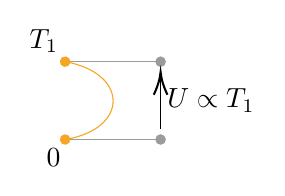
\begin{tikzpicture}[x=0.75pt,y=0.75pt,yscale=-1,xscale=1]
%uncomment if require: \path (0,110); %set diagram left start at 0, and has height of 110

%Straight Lines [id:da7792536568228223] 
\draw [color={rgb, 255:red, 155; green, 155; blue, 155 }  ,draw opacity=1 ]   (56.5,30) -- (102.5,30) ;
\draw [shift={(102.5,30)}, rotate = 0] [color={rgb, 255:red, 155; green, 155; blue, 155 }  ,draw opacity=1 ][fill={rgb, 255:red, 155; green, 155; blue, 155 }  ,fill opacity=1 ][line width=0.75]      (0, 0) circle [x radius= 2.01, y radius= 2.01]   ;
%Straight Lines [id:da7167294427341737] 
\draw [color={rgb, 255:red, 155; green, 155; blue, 155 }  ,draw opacity=1 ]   (56.5,67.5) -- (102.5,67.5) ;
\draw [shift={(102.5,67.5)}, rotate = 0] [color={rgb, 255:red, 155; green, 155; blue, 155 }  ,draw opacity=1 ][fill={rgb, 255:red, 155; green, 155; blue, 155 }  ,fill opacity=1 ][line width=0.75]      (0, 0) circle [x radius= 2.01, y radius= 2.01]   ;
%Straight Lines [id:da9591304964904978] 
\draw    (102.5,62.5) -- (102.5,37) ;
\draw [shift={(102.5,35)}, rotate = 450] [color={rgb, 255:red, 0; green, 0; blue, 0 }  ][line width=0.75]    (10.93,-3.29) .. controls (6.95,-1.4) and (3.31,-0.3) .. (0,0) .. controls (3.31,0.3) and (6.95,1.4) .. (10.93,3.29)   ;
%Curve Lines [id:da009398754899943462] 
\draw [color={rgb, 255:red, 245; green, 166; blue, 35 }  ,draw opacity=1 ]   (56.5,30) .. controls (87.33,35.5) and (87.33,62.5) .. (56.5,67.5) ;
\draw [shift={(56.5,67.5)}, rotate = 170.79] [color={rgb, 255:red, 245; green, 166; blue, 35 }  ,draw opacity=1 ][fill={rgb, 255:red, 245; green, 166; blue, 35 }  ,fill opacity=1 ][line width=0.75]      (0, 0) circle [x radius= 2.01, y radius= 2.01]   ;
\draw [shift={(56.5,30)}, rotate = 10.11] [color={rgb, 255:red, 245; green, 166; blue, 35 }  ,draw opacity=1 ][fill={rgb, 255:red, 245; green, 166; blue, 35 }  ,fill opacity=1 ][line width=0.75]      (0, 0) circle [x radius= 2.01, y radius= 2.01]   ;
% Text Node
\draw (54.5,27) node [anchor=south east] [inner sep=0.75pt]   [align=left] {$T_{1}$};
% Text Node
\draw (55.5,70.5) node [anchor=north east] [inner sep=0.75pt]   [align=left] {\SI{0}{\celsius}};
% Text Node
\draw (104.5,48.75) node [anchor=west] [inner sep=0.75pt]   [align=left] {$U \propto T_{1}$};
\end{tikzpicture}
\end{figure}
On peut déterminer $U$ à partir d'une température lorsqu'on connait précisément la mesure de $U$ à la valeur $T_2 = \SI{0}{\celsius}$. 
\end{exemple}

\subsubsection{Effet pyroélectrique}

Certains cristaux sont dits \emph{pyroélectriques} (le sulfate de triglycine par exemple) et présentent donc la propriété de présenter une polarisation électrique spontanée dépendant de la température du cristal. Ils comportent à leur surface des charges électriques $Q$ sur leurs surfaces et $-Q$ sur les surfaces opposées, proportionnelles à cette polarisation.



\begin{exemple}{Application de l'effet pyroélectrique}{}
~\\
\begin{figure}[H]

%lien d'édition des figures Tikz sur le site mathcha.io (rajouter le lien d'une modification effectuée sur la figure tikz avec le nom du modificateur car il n'y a qu'un lien par compte)

%lien mathcha Nom Prénom : https://www.mathcha.io/editor/5QmlWTYniVvh1nmzz0UV5K06oSl7KVnLfejoDdo


\tikzset{every picture/.style={line width=0.75pt}} %set default line width to 0.75pt        

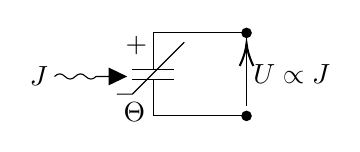
\begin{tikzpicture}[x=0.75pt,y=0.75pt,yscale=-1,xscale=1]
%uncomment if require: \path (0,110); %set diagram left start at 0, and has height of 110

%Straight Lines [id:da049441563073406525] 
\draw [color={rgb, 255:red, 0; green, 0; blue, 0 }  ,draw opacity=1 ]   (155,25) -- (200,25) ;
\draw [shift={(200,25)}, rotate = 0] [color={rgb, 255:red, 0; green, 0; blue, 0 }  ,draw opacity=1 ][fill={rgb, 255:red, 0; green, 0; blue, 0 }  ,fill opacity=1 ][line width=0.75]      (0, 0) circle [x radius= 2.01, y radius= 2.01]   ;
%Straight Lines [id:da0020140812998559188] 
\draw    (200,60) -- (200,32) ;
\draw [shift={(200,30)}, rotate = 450] [color={rgb, 255:red, 0; green, 0; blue, 0 }  ][line width=0.75]    (10.93,-3.29) .. controls (6.95,-1.4) and (3.31,-0.3) .. (0,0) .. controls (3.31,0.3) and (6.95,1.4) .. (10.93,3.29)   ;
%Straight Lines [id:da062183017724524614] 
\draw [color={rgb, 255:red, 0; green, 0; blue, 0 }  ,draw opacity=1 ]   (155,65) -- (200,65) ;
\draw [shift={(200,65)}, rotate = 0] [color={rgb, 255:red, 0; green, 0; blue, 0 }  ,draw opacity=1 ][fill={rgb, 255:red, 0; green, 0; blue, 0 }  ,fill opacity=1 ][line width=0.75]      (0, 0) circle [x radius= 2.01, y radius= 2.01]   ;
%Straight Lines [id:da18942991931898767] 
\draw    (145,42.5) -- (165,42.5) ;
%Straight Lines [id:da8438852563189819] 
\draw    (145,47.5) -- (165,47.5) ;
%Straight Lines [id:da5465187689829237] 
\draw    (155,25) -- (155,42.5) ;
%Straight Lines [id:da09145933722112254] 
\draw    (155,47.5) -- (155,65) ;

%Straight Lines [id:da8267186633709475] 
\draw    (137.5,54.5) -- (145,54.5) -- (170,29.5) ;
%Straight Lines [id:da7682659205660979] 
\draw    (107.5,46) .. controls (109.17,44.33) and (110.83,44.33) .. (112.5,46) .. controls (114.17,47.67) and (115.83,47.67) .. (117.5,46) .. controls (119.17,44.33) and (120.83,44.33) .. (122.5,46) .. controls (124.17,47.67) and (125.83,47.67) .. (127.5,46) -- (131.5,46) -- (139.5,46) ;
\draw [shift={(142.5,46)}, rotate = 180] [fill={rgb, 255:red, 0; green, 0; blue, 0 }  ][line width=0.08]  [draw opacity=0] (8.93,-4.29) -- (0,0) -- (8.93,4.29) -- cycle    ;

% Text Node
\draw (202,45) node [anchor=west] [inner sep=0.75pt]   [align=left] {$U \propto J$};
% Text Node
\draw (139.5,57.5) node [anchor=north west][inner sep=0.75pt]   [align=left] {$\Theta$};
% Text Node
\draw (140.5,25.5) node [anchor=north west][inner sep=0.75pt]   [align=left] {+};
% Text Node
\draw (105.5,46) node [anchor=east] [inner sep=0.75pt]   [align=left] {$J$};


\end{tikzpicture}

\end{figure}
On peut déterminer $U$ à partir d'un flux lumineux $J$ absorbé par un cristal pyroélectrique. Cela va élever sa température, ce qui entraîne une modification de sa polarisation qui est mesurable par la variation de tension $U$ aux bornes d'un condensateur associé.
\end{exemple}




\subsubsection{Effet piézoélectrique}

L'application d'une force ou d'une contrainte mécanique à certains matériaux dits piézoélectriques (le quartz par exemple) va entrainer une déformation provoquant l'apparition de charges électriques $Q$ sur leurs surfaces et $-Q$ sur leurs surfaces opposées.

\begin{exemple}{Application de l'effet piézoélectrique}{}
~\\
\begin{figure}[H]
\tikzset{every picture/.style={line width=0.75pt}} %set default line width to 0.75pt        

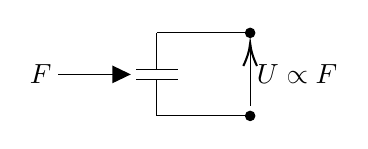
\begin{tikzpicture}[x=0.75pt,y=0.75pt,yscale=-1,xscale=1]
%uncomment if require: \path (0,110); %set diagram left start at 0, and has height of 110

%Straight Lines [id:da24742415739185752] 
\draw    (145,42.5) -- (165,42.5) ;
%Straight Lines [id:da5009949462555662] 
\draw    (145,47.5) -- (165,47.5) ;
%Straight Lines [id:da5246100942031141] 
\draw    (155,25) -- (155,42.5) ;
%Straight Lines [id:da18474784146966294] 
\draw    (155,47.5) -- (155,65) ;

%Straight Lines [id:da7890806725616728] 
\draw    (107.5,45) -- (139.5,45) ;
\draw [shift={(142.5,45)}, rotate = 180] [fill={rgb, 255:red, 0; green, 0; blue, 0 }  ][line width=0.08]  [draw opacity=0] (8.93,-4.29) -- (0,0) -- (8.93,4.29) -- cycle    ;
%Straight Lines [id:da3886370986269607] 
\draw [color={rgb, 255:red, 0; green, 0; blue, 0 }  ,draw opacity=1 ]   (155,25) -- (200,25) ;
\draw [shift={(200,25)}, rotate = 0] [color={rgb, 255:red, 0; green, 0; blue, 0 }  ,draw opacity=1 ][fill={rgb, 255:red, 0; green, 0; blue, 0 }  ,fill opacity=1 ][line width=0.75]      (0, 0) circle [x radius= 2.01, y radius= 2.01]   ;
%Straight Lines [id:da2942019649328115] 
\draw    (200,60) -- (200,32) ;
\draw [shift={(200,30)}, rotate = 450] [color={rgb, 255:red, 0; green, 0; blue, 0 }  ][line width=0.75]    (10.93,-3.29) .. controls (6.95,-1.4) and (3.31,-0.3) .. (0,0) .. controls (3.31,0.3) and (6.95,1.4) .. (10.93,3.29)   ;
%Straight Lines [id:da6965286794865602] 
\draw [color={rgb, 255:red, 0; green, 0; blue, 0 }  ,draw opacity=1 ]   (155,65) -- (200,65) ;
\draw [shift={(200,65)}, rotate = 0] [color={rgb, 255:red, 0; green, 0; blue, 0 }  ,draw opacity=1 ][fill={rgb, 255:red, 0; green, 0; blue, 0 }  ,fill opacity=1 ][line width=0.75]      (0, 0) circle [x radius= 2.01, y radius= 2.01]   ;
% Text Node
\draw (105.5,45) node [anchor=east] [inner sep=0.75pt]   [align=left] {$F$};
% Text Node
\draw (202,45) node [anchor=west] [inner sep=0.75pt]   [align=left] {$ U \propto F$};


\end{tikzpicture}
\end{figure}
On peut déterminer $U$ à partir d'une force $F$ (ou toutes grandeurs physiques dérivées) subie par l'élément piézoélectrique. Cela va provoquer une déformation de l'élément, ce qui entraine une modification de sa polarisation qui est mesurable par la variation de tension $U$ aux bornes d'un condensateur associé.
\end{exemple}


\subsubsection{Effet d'induction électromagnétique}

Lorsqu'un conducteur se déplace dans un \emph{champ magnétique} fixe $\overrightarrow{B}$, une \emph{tension} $U$ proportionnelle au \emph{flux d'induction magnétique} $\Phi$ par unité de temps $T$, et donc proportionnelle à sa vitesse de déplacement dans le champ d'induction magnétique $\overrightarrow{B}$.\\
Aussi, lorsqu'un circuit fermé est soumis à un flux d'induction magnétique $\Phi$ variable de par de son déplacement ou de celui de la source de l'induction (aimant par exemple), la tension $U$ dont il est le siège est égale au contraire de vitesse de variation du flux d'induction magnétique $\Phi$.



\begin{exemple}{Application de l'effet d'induction électromagnétique}{}
~\\
\begin{figure}[H]
\tikzset{every picture/.style={line width=0.75pt}} %set default line width to 0.75pt        

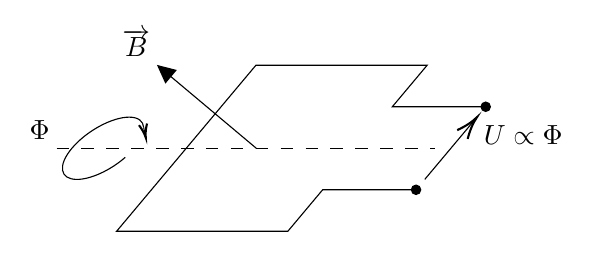
\begin{tikzpicture}[x=0.75pt,y=0.75pt,yscale=-1,xscale=1]
%uncomment if require: \path (0,156); %set diagram left start at 0, and has height of 156

%Straight Lines [id:da4159496238679624] 
\draw [color={rgb, 255:red, 0; green, 0; blue, 0 }  ,draw opacity=1 ]   (301.22,100) -- (256.22,100) -- (239.44,120) -- (156.94,120) -- (224.06,40) -- (306.56,40) -- (289.78,60) -- (334.78,60) ;
\draw [shift={(334.78,60)}, rotate = 0] [color={rgb, 255:red, 0; green, 0; blue, 0 }  ,draw opacity=1 ][fill={rgb, 255:red, 0; green, 0; blue, 0 }  ,fill opacity=1 ][line width=0.75]      (0, 0) circle [x radius= 2.01, y radius= 2.01]   ;
\draw [shift={(301.22,100)}, rotate = 180] [color={rgb, 255:red, 0; green, 0; blue, 0 }  ,draw opacity=1 ][fill={rgb, 255:red, 0; green, 0; blue, 0 }  ,fill opacity=1 ][line width=0.75]      (0, 0) circle [x radius= 2.01, y radius= 2.01]   ;
%Straight Lines [id:da9991618529346602] 
\draw    (305.41,95) -- (329.3,66.53) ;
\draw [shift={(330.59,65)}, rotate = 490] [color={rgb, 255:red, 0; green, 0; blue, 0 }  ][line width=0.75]    (10.93,-3.29) .. controls (6.95,-1.4) and (3.31,-0.3) .. (0,0) .. controls (3.31,0.3) and (6.95,1.4) .. (10.93,3.29)   ;
%Straight Lines [id:da8667170878421484] 
\draw  [dash pattern={on 4.5pt off 4.5pt}]  (128,80) -- (310.5,80) ;
%Shape: Arc [id:dp010359945518530145] 
\draw  [draw opacity=0] (161.1,84.37) .. controls (154.07,90.52) and (144.59,95) .. (137.83,95) .. controls (129.54,95) and (128.46,88.28) .. (135.41,80) .. controls (142.36,71.72) and (154.72,65) .. (163,65) .. controls (167.43,65) and (169.8,66.92) .. (169.98,69.97) -- (150.41,80) -- cycle ; \draw   (161.1,84.37) .. controls (154.07,90.52) and (144.59,95) .. (137.83,95) .. controls (129.54,95) and (128.46,88.28) .. (135.41,80) .. controls (142.36,71.72) and (154.72,65) .. (163,65) .. controls (167.43,65) and (169.8,66.92) .. (169.98,69.97) ;
%Straight Lines [id:da7991976387859124] 
\draw    (169.98,69.97) -- (170.6,72.94) ;
\draw [shift={(171.01,74.9)}, rotate = 258.2] [color={rgb, 255:red, 0; green, 0; blue, 0 }  ][line width=0.75]    (6.56,-1.97) .. controls (4.17,-0.84) and (1.99,-0.18) .. (0,0) .. controls (1.99,0.18) and (4.17,0.84) .. (6.56,1.97)   ;
%Straight Lines [id:da26501348792947876] 
\draw    (178.67,41.75) -- (224.25,80) ;
\draw [shift={(176.37,39.83)}, rotate = 40] [fill={rgb, 255:red, 0; green, 0; blue, 0 }  ][line width=0.08]  [draw opacity=0] (8.93,-4.29) -- (0,0) -- (8.93,4.29) -- cycle    ;

% Text Node
\draw (332.59,68) node [anchor=north west][inner sep=0.75pt]   [align=left] {$U \propto \Phi$};
% Text Node
\draw (174.37,36.83) node [anchor=south east] [inner sep=0.75pt]   [align=left] {$\overrightarrow{B}$};
% Text Node
\draw (126,77) node [anchor=south east] [inner sep=0.75pt]   [align=left] {$\Phi$};
\end{tikzpicture}
\end{figure}
La mesure de tension $U$ aux bornes du conducteur permet de déduire la vitesse de déplacement qui l'a induite.
\end{exemple}


\subsubsection{Effets photoélectriques}

Il existe plusieurs effets photoélectriques se distinguant par leurs manifestations mais ils ont tous comme point commun l'excitation de charges électriques dans la matière sous l'influence d'un rayonnement lumineux, dont la longueur d'onde est inférieure à une valeur seuil qui caractérise le matériau.

\begin{exemple}{Application de l'effet photoélectrique}{}
~\\
\begin{figure}[H]
\tikzset{every picture/.style={line width=0.75pt}} %set default line width to 0.75pt        

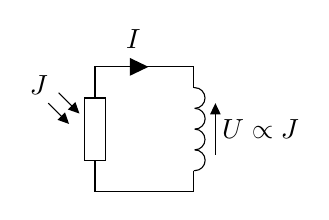
\begin{tikzpicture}[x=0.75pt,y=0.75pt,yscale=-1,xscale=1]
%uncomment if require: \path (0,153); %set diagram left start at 0, and has height of 153

%Straight Lines [id:da9553343306925111] 
\draw    (208,110.5) -- (208,115.5) ;
%Shape: Rectangle [id:dp7449879288789707] 
\draw   (213,80.5) -- (213,110.5) -- (203,110.5) -- (203,80.5) -- cycle ;
%Straight Lines [id:da5836322025533076] 
\draw    (208,75.5) -- (208,80.5) ;

%Straight Lines [id:da18940769793110568] 
\draw    (198.38,85.88) -- (190.5,78) ;
\draw [shift={(200.5,88)}, rotate = 225] [fill={rgb, 255:red, 0; green, 0; blue, 0 }  ][line width=0.08]  [draw opacity=0] (5.36,-2.57) -- (0,0) -- (5.36,2.57) -- cycle    ;
%Straight Lines [id:da5703289799533408] 
\draw    (193.38,90.88) -- (185.5,83) ;
\draw [shift={(195.5,93)}, rotate = 225] [fill={rgb, 255:red, 0; green, 0; blue, 0 }  ][line width=0.08]  [draw opacity=0] (5.36,-2.57) -- (0,0) -- (5.36,2.57) -- cycle    ;


%Straight Lines [id:da18160568852549952] 
\draw [color={rgb, 255:red, 0; green, 0; blue, 0 }  ,draw opacity=1 ]   (208,75.5) -- (208,65.5) -- (255.5,65.5) -- (255.5,75.5) ;
%Shape: Boxed Line [id:dp8550958962997346] 
\draw [color={rgb, 255:red, 0; green, 0; blue, 0 }  ,draw opacity=1 ]   (255.5,115.5) -- (255.5,125.5) -- (208,125.5) -- (208,115.5) ;
%Shape: Arc [id:dp9236278998461147] 
\draw  [draw opacity=0] (255.71,75.51) .. controls (255.81,75.5) and (255.9,75.5) .. (256,75.5) .. controls (258.76,75.5) and (261,77.74) .. (261,80.5) .. controls (261,83.25) and (258.78,85.48) .. (256.04,85.5) -- (256,80.5) -- cycle ; \draw   (255.71,75.51) .. controls (255.81,75.5) and (255.9,75.5) .. (256,75.5) .. controls (258.76,75.5) and (261,77.74) .. (261,80.5) .. controls (261,83.25) and (258.78,85.48) .. (256.04,85.5) ;
%Shape: Arc [id:dp01043642876607509] 
\draw  [draw opacity=0] (256.04,85.5) .. controls (256.05,85.5) and (256.05,85.5) .. (256.06,85.5) .. controls (258.82,85.5) and (261.06,87.74) .. (261.06,90.5) .. controls (261.06,93.25) and (258.84,95.48) .. (256.1,95.5) -- (256.06,90.5) -- cycle ; \draw   (256.04,85.5) .. controls (256.05,85.5) and (256.05,85.5) .. (256.06,85.5) .. controls (258.82,85.5) and (261.06,87.74) .. (261.06,90.5) .. controls (261.06,93.25) and (258.84,95.48) .. (256.1,95.5) ;
%Shape: Arc [id:dp6271751911575147] 
\draw  [draw opacity=0] (255.98,95.5) .. controls (255.99,95.5) and (255.99,95.5) .. (256,95.5) .. controls (258.76,95.5) and (261,97.74) .. (261,100.5) .. controls (261,103.25) and (258.78,105.48) .. (256.04,105.5) -- (256,100.5) -- cycle ; \draw   (255.98,95.5) .. controls (255.99,95.5) and (255.99,95.5) .. (256,95.5) .. controls (258.76,95.5) and (261,97.74) .. (261,100.5) .. controls (261,103.25) and (258.78,105.48) .. (256.04,105.5) ;
%Shape: Arc [id:dp7604597461390405] 
\draw  [draw opacity=0] (256.04,105.5) .. controls (256.05,105.5) and (256.05,105.5) .. (256.06,105.5) .. controls (258.82,105.5) and (261.06,107.74) .. (261.06,110.5) .. controls (261.06,113.26) and (258.82,115.5) .. (256.06,115.5) .. controls (255.9,115.5) and (255.74,115.49) .. (255.59,115.48) -- (256.06,110.5) -- cycle ; \draw   (256.04,105.5) .. controls (256.05,105.5) and (256.05,105.5) .. (256.06,105.5) .. controls (258.82,105.5) and (261.06,107.74) .. (261.06,110.5) .. controls (261.06,113.26) and (258.82,115.5) .. (256.06,115.5) .. controls (255.9,115.5) and (255.74,115.49) .. (255.59,115.48) ;

%Straight Lines [id:da7979642956460348] 
\draw    (266,86) -- (266,108) ;
\draw [shift={(266,83)}, rotate = 90] [fill={rgb, 255:red, 0; green, 0; blue, 0 }  ][line width=0.08]  [draw opacity=0] (5.36,-2.57) -- (0,0) -- (5.36,2.57) -- cycle    ;
%Straight Lines [id:da6970578975487184] 
\draw    (232.75,65.5) -- (255.5,65.5) ;
\draw [shift={(233.75,65.5)}, rotate = 180] [fill={rgb, 255:red, 0; green, 0; blue, 0 }  ][line width=0.08]  [draw opacity=0] (8.93,-4.29) -- (0,0) -- (8.93,4.29) -- cycle    ;

% Text Node
\draw (186.5,80) node [anchor=south east] [inner sep=0.75pt]   [align=left] {$J$};
% Text Node
\draw (268,95.5) node [anchor=west] [inner sep=0.75pt]   [align=left] {$U \propto J$};
% Text Node
\draw (226.5,58) node [anchor=south] [inner sep=0.75pt]   [align=left] {$I$};


\end{tikzpicture}
\end{figure}
Les effets photoélectriques permettent d'obtenir une tension $U$ ou un courant $I$ en fonction du rayonnement lumineux $J$ du matériau. D'une part, ils constituent la base des méthodes de mesure des grandeurs photométriques, d'autre part, ils permettent la traduction en signal électriques des informations véhiculées par un rayonnement lumineux.
\end{exemple}



\subsubsection{Effets photoémissif}

Les électrons libérés sont émis hors d'une zone éclairée et, lors de l'application d'un champ électrique, forment un courant électrique.

\subsubsection{Effets photovoltaïque}

Des électrons et des trous pouvant recevoir des électrons sont libérés au voisinage de la jonction Positive Négative (PN) d'un semi-conducteur éclairée. Leur déplacement dans le champ électrique de la jonction PN module la tension aux bornes de cette jonction.

\subsubsection{Effet photoélectromagnétique}

L'application d'un champ magnétique perpendiculaire à un rayonnement lumineux va provoquer dans le matériaux éclairé l'apparition d'une tension électrique dans la direction \emph{normale} au champ magnétique et au rayonnement.

\subsubsection{Effet Hall}

Un matériau, de préférence semi-conducteur et sous forme de plaquette, fait apparaitre une tension $v_{H}$ lorsqu'il est parcouru par un courant $I$ et soumis à un champ magnétique $\overrightarrow{B}$ d'un angle $\theta$ avec le courant $I$.

\begin{formule}{Effet Hall}{effet_hall}
\begin{align*}
v_H &= K_H \times I \times B \times \sin\theta
\end{align*}

\begin{textvariables}
\K_H							& coefficient	& 				& 		/											& 	Facteur dépendant du matériau et de la dimension de la plaquette \\
I									& intensité		& 	ampère			& 		\ampere					& Source de courant fournissant l'énergie liée au signal de sortie  \\
\overrightarrow{B}									& champ magnétique		& Tesla		& \tesla						& Champ magnétique soumis au matériau \\
\sin\theta					& angle							& radian		& \radian				& Angle formé par l'intensité $I$ et le champ magnétique $\overrightarrow{B}$ \\
\end{textvariables}
\end{formule}


\begin{exemple}{Application de l'effet Hall}{}
~\\
\begin{figure}[H]

\tikzset{every picture/.style={line width=0.75pt}} %set default line width to 0.75pt        

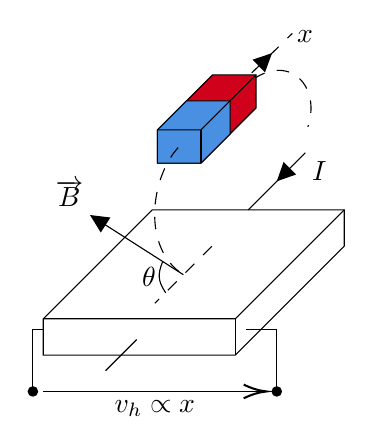
\begin{tikzpicture}[x=0.75pt,y=0.75pt,yscale=-1,xscale=1]
%uncomment if require: \path (0,255); %set diagram left start at 0, and has height of 255

%Curve Lines [id:da026480600050421743] 
\draw  [dash pattern={on 4.5pt off 4.5pt}]  (390,37.5) .. controls (411.6,12.4) and (432.3,30.3) .. (425,52.5) ;
%Shape: Cube [id:dp07360762187167524] 
\draw  [fill={rgb, 255:red, 208; green, 2; blue, 27 }  ,fill opacity=1 ] (352.5,54.06) -- (379.06,27.5) -- (400,27.5) -- (400,43.44) -- (373.44,70) -- (352.5,70) -- cycle ; \draw   (400,27.5) -- (373.44,54.06) -- (352.5,54.06) ; \draw   (373.44,54.06) -- (373.44,70) ;
%Shape: Cube [id:dp18529556990685714] 
\draw  [fill={rgb, 255:red, 74; green, 144; blue, 226 }  ,fill opacity=1 ] (352.5,54) -- (366.5,40) -- (387.5,40) -- (387.5,56) -- (373.5,70) -- (352.5,70) -- cycle ; \draw   (387.5,40) -- (373.5,54) -- (352.5,54) ; \draw   (373.5,54) -- (373.5,70) ;

%Shape: Cube [id:dp5559755925236529] 
\draw   (297.5,145) -- (350,92.5) -- (442.5,92.5) -- (442.5,110) -- (390,162.5) -- (297.5,162.5) -- cycle ; \draw   (442.5,92.5) -- (390,145) -- (297.5,145) ; \draw   (390,145) -- (390,162.5) ;
%Straight Lines [id:da7084755043157218] 
\draw    (327.5,170) -- (342.5,155) ;
%Straight Lines [id:da9878757017878151] 
\draw    (396.25,92.5) -- (423.75,65) ;
\draw [shift={(410,78.75)}, rotate = 315] [fill={rgb, 255:red, 0; green, 0; blue, 0 }  ][line width=0.08]  [draw opacity=0] (8.93,-4.29) -- (0,0) -- (8.93,4.29) -- cycle    ;
%Straight Lines [id:da6115380075011939] 
\draw    (297.5,145) -- (390,145) ;
%Straight Lines [id:da8865101665838837] 
\draw  [dash pattern={on 4.5pt off 4.5pt}]  (378.75,110) -- (351.25,137.5) ;
%Straight Lines [id:da4151864093884584] 
\draw    (322.53,96.62) -- (365,123.75) ;
\draw [shift={(320,95)}, rotate = 32.57] [fill={rgb, 255:red, 0; green, 0; blue, 0 }  ][line width=0.08]  [draw opacity=0] (8.93,-4.29) -- (0,0) -- (8.93,4.29) -- cycle    ;
%Straight Lines [id:da13161923838594092] 
\draw  [dash pattern={on 4.5pt off 4.5pt}]  (397.97,26.5) -- (417.5,7.5) ;
\draw [shift={(407.73,17)}, rotate = 495.79] [fill={rgb, 255:red, 0; green, 0; blue, 0 }  ][line width=0.08]  [draw opacity=0] (8.93,-4.29) -- (0,0) -- (8.93,4.29) -- cycle    ;
%Curve Lines [id:da8220459438720412] 
\draw  [dash pattern={on 4.5pt off 4.5pt}]  (362.5,62.5) .. controls (349.4,76.7) and (344.6,110.7) .. (365,123.75) ;
%Curve Lines [id:da48302895341966623] 
\draw    (355,117.5) .. controls (352.6,123.5) and (352.6,126.7) .. (356.5,132.5) ;
%Straight Lines [id:da0016723825185572805] 
\draw    (410,180) -- (410,150) -- (395,150) ;
\draw [shift={(410,180)}, rotate = 270] [color={rgb, 255:red, 0; green, 0; blue, 0 }  ][fill={rgb, 255:red, 0; green, 0; blue, 0 }  ][line width=0.75]      (0, 0) circle [x radius= 2.01, y radius= 2.01]   ;
%Straight Lines [id:da6665646722680143] 
\draw    (292.5,180) -- (292.5,150) -- (297.5,150) ;
\draw [shift={(292.5,180)}, rotate = 270] [color={rgb, 255:red, 0; green, 0; blue, 0 }  ][fill={rgb, 255:red, 0; green, 0; blue, 0 }  ][line width=0.75]      (0, 0) circle [x radius= 2.01, y radius= 2.01]   ;
%Straight Lines [id:da45157029340764043] 
\draw    (297.5,180) -- (403,180) ;
\draw [shift={(405,180)}, rotate = 180] [color={rgb, 255:red, 0; green, 0; blue, 0 }  ][line width=0.75]    (10.93,-3.29) .. controls (6.95,-1.4) and (3.31,-0.3) .. (0,0) .. controls (3.31,0.3) and (6.95,1.4) .. (10.93,3.29)   ;

% Text Node
\draw (425.75,68) node [anchor=north west][inner sep=0.75pt]   [align=left] {$I$};
% Text Node
\draw (318,92) node [anchor=south east] [inner sep=0.75pt]   [align=left] {$\overrightarrow{B}$};
% Text Node
\draw (353,125) node [anchor=east] [inner sep=0.75pt]   [align=left] {$\theta$};
% Text Node
\draw (418.5,5) node [anchor=north west][inner sep=0.75pt]   [align=left] {$x$};
% Text Node
\draw (351.25,183) node [anchor=north] [inner sep=0.75pt]   [align=left] {$v_{h} \propto x$};

\end{tikzpicture}
\end{figure}
Pour connaître la position de l'objet, on lui accouple un aimant qui va lui déterminer les valeurs de $\overrightarrow{B}$ et $\theta$ au niveau de la plaquette. La tension $v_{h}$ aux bornes de la plaquette est donc fonction de cet aimant et permet une conversion électrique d'une position $x$.
\end{exemple}



Il convient de classer les capteurs basés sur l'effet Hall parmi les capteurs actifs puisque l'information sortie est liée à une tension $v_H$, quand bien même il ne s'agit pas de \emph{convertisseurs d'énergie} car c'est une source de courant $I$  et non le mesurande qui va délivrer l'énergie liée au signal de sortie.

\subsection{Capteurs passifs}

Les capteurs passifs sont donc des \emph{récepteurs} qui vont voir leurs grandeurs physiques être modulées par le mesurande sans pour autant convertir une énergie. On distingue dans les récepteurs plusieurs grandeurs physiques liées à :
\begin{itemize}
\item leur géométrie et leurs dimensions\,;
\item leurs propriétés électriques :
\begin{itemize}
\item résistivité $\rho$\,;
\item perméabilité magnétique $\mu$\,;
\item constante diélectrique $\varepsilon$.
\end{itemize}
\end{itemize}

Un mesurande module donc sur la variation du signal de sortie électrique du capteur passif :
\begin{itemize}
\item soit par les caractéristiques géométriques ou des dimensions\,;
\item soit par les propriétés électriques des matériaux\,;
\item soit plus rarement par les deux à la fois.
\end{itemize}

\subsubsection{Paramètres géométrique et dimensionnel du capteur passif}

Pour que les paramètres géométriques ou dimensionnels du capteur passif puissent varier, il faut que le capteur comporte des éléments mobiles ou déformables.\\

\paragraph{Position}

Le principe d'une majorité de capteurs de déplacement et de position se base sur un élément mobile du capteur qui présente des positions spécifiques pour des valeurs de sorties précises. La mesure de cette valeur de sortie permet de connaître la position de l'élément mobile (potentiomètre, condensateur à armature mobile, inductance à noyau mobile\ldots).

\paragraph{Déformation}

La déformation est la résultante de forces -- ou de grandeurs dérivées --  qui est appliquée directement ou indirectement sur un capteur (armature d'un condensateur soumis à une pression différentielle, jauge d'extensométrie liée de manière rigide à une structure contrainte\ldots).\\
Cela entraine une modification du signal du sortie $s$, qui sera corrélée à la valeur de la force appliquée sur le capteur.

\paragraph{Propriétés électriques des matériaux}

Les propriétés électriques des matériaux varient selon leur nature et sont également sensibles à diverses grandeurs physiques (température, pression, humidité, éclairement\ldots).\\
Dans le cas ou seule l'une de ces grandeurs est susceptible de modifier les propriétés électriques d'un matériau mais que les autres n'influencent pas ces mêmes propriétés, il s'établit alors une corrélation entre ces cette grandeur physique et le signal de sortie $s$.

\begin{table}[H]
\caption{Capteurs passifs principaux selon les effets physiques}

\begin{tabularx}{\linewidth}{XX>{\compress}X}
\toprule
\thead{Mesurande}						&	\thead{Caractéristique électrique sensible}					&	\thead{Matériau utilisé} \\
\midrule
Température									& Résistivité						& 
\begin{tabitemize}
\item métaux (platine, cuivre, nickel)\,;
\item semi-conducteurs.
\end{tabitemize}
 \\
 Très basse température				& Constante diélectrique				& Verre \\
\addlinespace
Flux de rayonnement optique			& Résistivité									& Semi-conducteurs \\
\addlinespace
Déformation									& 	Résistivité		 											& \begin{tabitemize}
\item alliages de nickel\,;
\item silicium dopé.
\end{tabitemize}
 \\
													& 	Perméabilité magnétique						& 	Alliages ferromagnétiques		 \\
\addlinespace
Position (aimant)											& 	Résistivité		& 	Matériaux magnéto-résistant (bismuth, antimoniure d'indium)		 \\
\addlinespace
Humidité									&  Résistivité													& 	Chlorure de lithium		 \\
									&  Constante diélectrique								& 	Alumine, polymères		 \\
\addlinespace
Niveau							& 	Constante diélectrique								& Liquides isolants \\
\bottomrule
\end{tabularx}
\end{table}

Dans le tableau ci-dessus, on remarque l'importe de la propriété de la \emph{résistivité} $\rhoup$.\\
Le signal de sortie $s$ des \emph{capteurs passifs} n'est mesurable qu'en intégrant le capteur dans un circuit électrique alimenté, désigné comme étant son \emph{conditionneur}. Ils en existe plusieurs sortes dont les principaux sont les suivants :
\begin{description}
\item [montage potentiométrique :] association \emph{en série} d'un capteur et d'une impédance pouvant être ou non du même type\,;
\item [pont d'impédances :] équilibre électrique du pont permettant la détermination de l'impédance de sortie du capteur ou déséquilibre du pont permettant la mesure de la variation de cette impédance\,;
\item [circuit oscillant :] circuit contenant l'impédance du capteur et faisant partie d'un circuit oscillateur dont il détermine la fréquence\,;
\item [amplificateur opérationnel :] circuit dont l'impédance du capteur constitue l'un des éléments déterminant le gain de l'amplificateur.
\end{description}

Choisir un \emph{conditionneur} est une étape primordiale dans la réalisation de mesures. L'association d'un capteur et de son conditionneur -- dont sa constitution -- déterminera le signal électrique et en découleront un bon nombre de performances de mesures :
\begin{itemize}
\item sensibilité\,;
\item linéarité\,;
\item insensibilité à certaines grandeurs d'influences.
\end{itemize}

\section{Corps d'épreuves et capteurs composites}

Pour certaines raisons (coût, facilité d'exploitation\ldots), on peut utiliser des capteur sensible à l'un des effets du \emph{mesurande} plutôt qu'au mesurande lui-même.

\begin{definition}{Corps d'épreuve}{}
Dispositif de mesure qui, une fois soumis à un mesurande désigné \emph{mesurande primaire} dont il faut connaitre la grandeur, assure la traduction en une autre grandeur physique non-électrique désignée \emph{mesurande secondaire}.
\end{definition}
\begin{definition}{Capteur composite}{}
Ensemble formé par le corps d'épreuve et un capteur passif ou actif nécessaire à la traduction du mesurande secondaire donnée par le corps d'épreuve.
\end{definition}

%--------------------------------------
%CANEVAS
%--------------------------------------

%utiliser les environnement \begin{comment} \end{comment} pour mettre en commentaire le préambule une fois la programmation appelée dans le document maître (!ne pas oublier de mettre en commentaire \end{document}!)

\begin{comment}

\documentclass[a4paper, 11pt, twoside, fleqn]{memoir}

\usepackage{AOCDTF}

\marqueurchapitre
\decoupagechapitre{1} %juste pour éviter les erreurs lors de la compilation des sous-programmations (passera en commentaire)

%lien d'édition des figures Tikz sur le site mathcha.io (rajouter le lien d'une modification effectuée sur la figure tikz avec le nom du modificateur car il n'y a qu'un lien par compte) 

%lien mathcha Nom Prénom : https://www.mathcha.io/editor/88XmJTWQUxztLv21v6S12z22Lf78mx9yIOvQ9M5

%--------------------------------------
%corps du document
%--------------------------------------

\begin{document} %corps du document
	\openleft %début de chapitre à gauche

\end{comment}

\begin{figure}[h]
\caption{Structure d'un corps d'épreuve}

\tikzset{every picture/.style={line width=0.75pt}} %set default line width to 0.75pt        

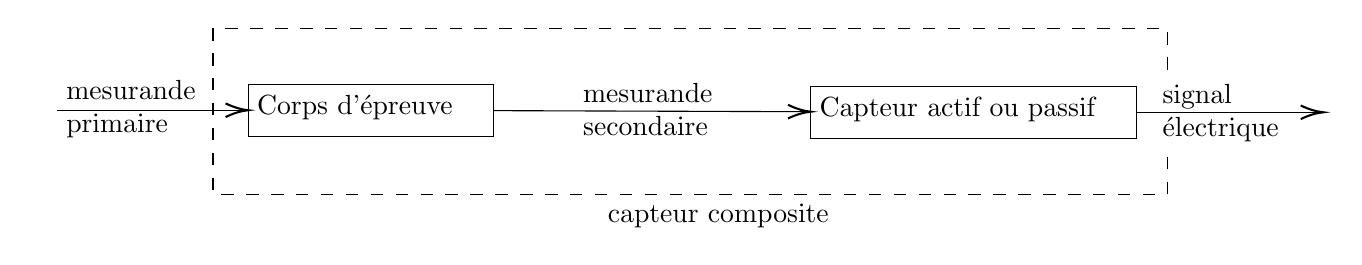
\begin{tikzpicture}[x=0.75pt,y=0.75pt,yscale=-1,xscale=1]
%uncomment if require: \path (0,300); %set diagram left start at 0, and has height of 300

%Straight Lines [id:da6331649314862131] 
\draw  [dash pattern={on 4.5pt off 4.5pt}]  (550,120) -- (550,100) -- (90,100) -- (90,180) -- (550,180) -- (550,160) ;

% Text Node
\draw    (107,127) -- (225,127) -- (225,152) -- (107,152) -- cycle  ;
\draw (110,131) node [anchor=north west][inner sep=0.75pt]   [align=left] {Corps d'épreuve};
% Text Node
\draw    (378,128) -- (535,128) -- (535,153) -- (378,153) -- cycle  ;
\draw (381,132) node [anchor=north west][inner sep=0.75pt]   [align=left] {Capteur actif ou passif};
% Text Node
\draw (1,131) node [anchor=north west][inner sep=0.75pt]   [align=left] {};
% Text Node
\draw (50.5,139) node   [align=left] {mesurande\\primaire};
% Text Node
\draw (299.5,139) node   [align=left] {mesurande\\secondaire};
% Text Node
\draw (628,132) node [anchor=north west][inner sep=0.75pt]   [align=left] {};
% Text Node
\draw (575.5,141) node   [align=left] {signal\\électrique};
% Text Node
\draw (333.5,190.5) node   [align=left] {capteur composite};
% Connection
\draw    (225,139.7) -- (376,140.22) ;
\draw [shift={(378,140.23)}, rotate = 180.2] [color={rgb, 255:red, 0; green, 0; blue, 0 }  ][line width=0.75]    (10.93,-3.29) .. controls (6.95,-1.4) and (3.31,-0.3) .. (0,0) .. controls (3.31,0.3) and (6.95,1.4) .. (10.93,3.29)   ;
% Connection
\draw    (15,139.5) -- (105,139.5) ;
\draw [shift={(107,139.5)}, rotate = 180] [color={rgb, 255:red, 0; green, 0; blue, 0 }  ][line width=0.75]    (10.93,-3.29) .. controls (6.95,-1.4) and (3.31,-0.3) .. (0,0) .. controls (3.31,0.3) and (6.95,1.4) .. (10.93,3.29)   ;
% Connection
\draw    (535,140.5) -- (623,140.5) ;
\draw [shift={(625,140.5)}, rotate = 180] [color={rgb, 255:red, 0; green, 0; blue, 0 }  ][line width=0.75]    (10.93,-3.29) .. controls (6.95,-1.4) and (3.31,-0.3) .. (0,0) .. controls (3.31,0.3) and (6.95,1.4) .. (10.93,3.29)   ;

\end{tikzpicture}
\end{figure}

%\end{document}



\begin{exemple}{Application d'un capteur composite}{}
Une force de traction $F$ est appliquée sur un objet d'une section $S$ et d'une longueur $L$, qui va subir un allongement de sa longueur $\frac{\Delta L}{L}$, entrainant de ce fait une variation de la résistance d'une jauge \Circled{1} d'un facteur $K$ placée sur l'objet $\frac{\Delta R}{R}$.
\begin{formule*}{Module de Young}{}
\begin{align*}
		E 	&= \frac{\varepsilon}{\sigma}
\end{align*}
\begin{textvariables}
E 					& Pression		&	Pascal			& \pascal 				& Module de Young (de traction) d'un matérieau \emph{élastique} et \emph{isotope} \\ 
\varepsilon	& Mètre			& 	Mètre			& \meter				& Allongement relatif (déformation) $\frac{\Delta L}{L}$ \\
 \sigma			& Pression		&	Pascal			& \pascal				& contrainte sur le matériau \\
\end{textvariables}
\end{formule*}

\begin{center}
%https://www.mathcha.io/editor/Gq5WKTE5SOVh1Y2BNvf3MWGXJHB9DB8dFlvmpqK
% Pattern Info
 
\tikzset{
pattern size/.store in=\mcSize, 
pattern size = 5pt,
pattern thickness/.store in=\mcThickness, 
pattern thickness = 0.3pt,
pattern radius/.store in=\mcRadius, 
pattern radius = 1pt}
\makeatletter
\pgfutil@ifundefined{pgf@pattern@name@_23ewa924x}{
\pgfdeclarepatternformonly[\mcThickness,\mcSize]{_23ewa924x}
{\pgfqpoint{0pt}{0pt}}
{\pgfpoint{\mcSize+\mcThickness}{\mcSize+\mcThickness}}
{\pgfpoint{\mcSize}{\mcSize}}
{
\pgfsetcolor{\tikz@pattern@color}
\pgfsetlinewidth{\mcThickness}
\pgfpathmoveto{\pgfqpoint{0pt}{0pt}}
\pgfpathlineto{\pgfpoint{\mcSize+\mcThickness}{\mcSize+\mcThickness}}
\pgfusepath{stroke}
}}
\makeatother
\tikzset{every picture/.style={line width=0.5pt}} %set default line width to 0.75pt        

\begin{tikzpicture}[x=0.75pt,y=0.75pt,yscale=-0.6,xscale=0.6]
%uncomment if require: \path (0,300); %set diagram left start at 0, and has height of 300

%Shape: Can [id:dp12472449649523132] 
\draw   (134.92,100) -- (345.08,100) .. controls (350.56,100) and (355,113.43) .. (355,130) .. controls (355,146.57) and (350.56,160) .. (345.08,160) -- (134.92,160) .. controls (129.44,160) and (125,146.57) .. (125,130) .. controls (125,113.43) and (129.44,100) .. (134.92,100) .. controls (140.39,100) and (144.83,113.43) .. (144.83,130) .. controls (144.83,146.57) and (140.39,160) .. (134.92,160) ;
%Straight Lines [id:da5161240947796851] 
\draw    (135,130) -- (98,130) ;
\draw [shift={(95,130)}, rotate = 360] [fill={rgb, 255:red, 0; green, 0; blue, 0 }  ][line width=0.08]  [draw opacity=0] (8.93,-4.29) -- (0,0) -- (8.93,4.29) -- cycle    ;
%Straight Lines [id:da28806277731694174] 
\draw    (382,130) -- (355,130) ;
\draw [shift={(385,130)}, rotate = 180] [fill={rgb, 255:red, 0; green, 0; blue, 0 }  ][line width=0.08]  [draw opacity=0] (8.93,-4.29) -- (0,0) -- (8.93,4.29) -- cycle    ;
%Straight Lines [id:da3487762389054402] 
\draw  [dash pattern={on 4.5pt off 4.5pt}]  (134.92,165) -- (135,185) ;
%Straight Lines [id:da07803041607897865] 
\draw  [dash pattern={on 4.5pt off 4.5pt}]  (344.92,165) -- (345,185) ;
%Straight Lines [id:da4638976844778334] 
\draw    (137,185) -- (343,185) ;
\draw [shift={(345,185)}, rotate = 180] [color={rgb, 255:red, 0; green, 0; blue, 0 }  ][line width=0.75]    (10.93,-3.29) .. controls (6.95,-1.4) and (3.31,-0.3) .. (0,0) .. controls (3.31,0.3) and (6.95,1.4) .. (10.93,3.29)   ;
\draw [shift={(135,185)}, rotate = 0] [color={rgb, 255:red, 0; green, 0; blue, 0 }  ][line width=0.75]    (10.93,-3.29) .. controls (6.95,-1.4) and (3.31,-0.3) .. (0,0) .. controls (3.31,0.3) and (6.95,1.4) .. (10.93,3.29)   ;
%Shape: Ellipse [id:dp48131477454456484] 
\draw  [pattern=_23ewa924x,pattern size=6pt,pattern thickness=0.75pt,pattern radius=0pt, pattern color={rgb, 255:red, 0; green, 0; blue, 0}] (125,130) .. controls (125,113.43) and (129.44,100) .. (134.92,100) .. controls (140.39,100) and (144.83,113.43) .. (144.83,130) .. controls (144.83,146.57) and (140.39,160) .. (134.92,160) .. controls (129.44,160) and (125,146.57) .. (125,130) -- cycle ;
%Shape: Rectangle [id:dp9836272663606409] 
\draw  [fill={rgb, 255:red, 0; green, 0; blue, 0 }  ,fill opacity=1 ] (240,152.5) -- (270,152.5) -- (270,160) -- (240,160) -- cycle ;

% Text Node
\draw (93,130) node [anchor=east] [inner sep=0.75pt]   [align=left] {$F$};
% Text Node
\draw (387,130) node [anchor=west] [inner sep=0.75pt]   [align=left] {$F$};
% Text Node
\draw (240,188) node [anchor=north] [inner sep=0.75pt]   [align=left] {$L$};
% Text Node
\draw (91,65) node [anchor=north west][inner sep=0.75pt]   [align=left] {$S$};
% Text Node
\draw (134.92,130) node   [align=left] {};
% Text Node
\draw (272,149.5) node [anchor=south west] [inner sep=0.75pt]   [align=left] {\Circled{1}};
% Connection
\draw    (105,86.39) -- (125.29,115.96) ;
\draw [shift={(126.42,117.61)}, rotate = 235.55] [color={rgb, 255:red, 0; green, 0; blue, 0 }  ][line width=0.75]    (10.93,-3.29) .. controls (6.95,-1.4) and (3.31,-0.3) .. (0,0) .. controls (3.31,0.3) and (6.95,1.4) .. (10.93,3.29)   ;

\end{tikzpicture}
\end{center}


Dans l'exemple la relation entre le mesurande primaire, la traction $F$ et le mesurande secondaire, la déformation $\frac{\Delta L}{L}$, est :
\begin{align*}
\frac{\Delta L}{L} &= \frac{1}{E} \times \frac{F}{S} 
\end{align*}
D'autre part, la relation entre la grandeur de sortie, la variation de la résistance de la jauge $\frac{\Delta R}{R}$ et le mesurande secondaire, la déformation $\frac{\Delta L}{L}$ est :
\begin{align*}
\frac{\Delta R}{R} &= K \times \frac{\Delta L}{L}
\end{align*}
La relation de la variation de la résistance de la jauge $R$ et la traction :
\begin{align*}
\frac{\Delta R}{R} &= \frac{K}{E} \times \frac{F}{S} 
\end{align*}
\end{exemple}

Les corps d'épreuves sont très utilisés pour mesurer des grandeurs physiques en mécanique.\\
La relation entre le mesurande primaire et le mesurande secondaire est très souvent linéaire, en particulier dans le cas de déformations et déplacement résultants de contraintes mécaniques, dans les conditions limites de l'élasticité du corps d'épreuve. Les performances de l'association corps d'épreuve -- capteur doivent être déterminées par un étalonnage tenant compte des éventuelles conséquences de leur liaison par rapport à leurs caractéristiques individuelles.\\
Si de l'électronique est intégrée au capteur, il s'agira d'un \emph{capteur intégré}.

\section{Grandeurs d'influence}

Un capteur se situe dans un environnement qui le soumet à un mesurande mais également à d'autres grandeurs physiques susceptibles de biaiser la valeur de la grandeur de sortie, sans distinction d'origine du biais.

\begin{definition}{Grandeur d'influence}{}
Grandeur physique \og parasite \fg{} à laquelle la réponse d'un capteur peut être sensible.
\end{definition}

On distingue par exemple :
\begin{itemize}
\item température pouvant faire varier la réponse d'un capteur optique\,;
\item champ magnétique pouvant faire varier la réponse d'un capteur thermométrique.
\end{itemize}

Les principales grandeurs d'influences sont :
\begin{description}
\item [température :] modification des caractéristiques électriques, mécaniques et dimensionnelles des composants du capteur\,;
\item [pression, accélération, vibration :] perturbations pouvant créer des déformations et des contraintes dans certains composants du capteur, altérant ainsi sa réponse\,;
\item [humidité :] dégradation de l'isolation (capteur/environnement et composant du capteur) et perturbation de certaines propriétés électriques (constante diélectrique, résistivité\ldots)\,;
\item [champs magnétiques variables et statiques :] apparition potentielle de tension induite pouvant se superposer au signal utile en régime statique et modification des propriété électrique en régime variable\,;
\item [tension d'alimentation (amplitude et fréquence) :] grandeur de sortie du capteur dépendante de ces grandeurs de par le principe même du capteur.
\end{description}

Si l'on se réfère à la relation mesurande -- grandeur de sortie (\superref{form:grandeur_sortie}) et qu'on comptabilise l'influence de $g_1$, $g_2$\ldots, cela donne :
\begin{formule}{Grandeurs d'influence}{grandeurs_influences}
\begin{align*}
   		s &= F(m, g_1, g_2\ldots) \\
\end{align*}

\begin{textvariables}
s						& grandeur électrique	& 			& 		/					& 	Grandeur (réponse) de sortie de nature électrique (charge, tension, courant ou impédance) fonction du mesurande \\
m						& grandeur physique		& 			& 		/					& Grandeur physique d'entrée d'excitation autre qu'électrique  \\
g_1					& grandeur physique		& 			& 		/					& Grandeur physique d'influence 1  \\
g_2					& grandeur physique		& 			& 		/					& Grandeur physique d'influence 2  \\
\end{textvariables}
\end{formule}

Pour déduire la valeur de $s$ en fonction de $m$ seul, il convient de :
\begin{itemize}
\item soit de réduire l'importance des grandeurs d'influence au niveau du capteur en le protégeant par un isolement adéquat (supports antivibratoires, blindages magnétiques\ldots)\,;
\item soit de stabiliser ces grandeurs d'influences à des seuils précisément déterminés et d'étalonner le capteur dans ces conditions de fonctionnement (enceinte climatique, sources d'alimentation régulées\ldots)\,;
\item soit d'utiliser un montage pouvant compenser l'influence des perturbations. 
\end{itemize}

\section{Chaine de mesure}

\begin{definition}{Chaine de mesure}{}
Ensemble des dispositifs, y compris le capteur, dont le but est de délivrer la détermination précise de la valeur d'un mesurande dans les meilleures conditions.  
\end{definition}

En entrée de chaine, le capteur est soumis à l'action du mesurande $m$ et injectera son signal de sortie $s$ dans la chaine. En fin de chaine, le signal de sortie $s$ est converti pour rendre la lecture de la valeur du mesurande $m$ possible.
C'est l'étalonnage de la chaine de mesure dans son ensemble qui déterminera au mieux la valeur de sortie $s$ par rapport au mesurande $m$ correspondant. \\
La chaine de mesure comprend le capteur (avec son conditionneur s'il est passif) associé à un appareil de lecture dans sa forme la plus simple (thermocouple et voltmètre par exemple).\\
Toutefois, les exigences requises par les conditions d'exploitation et la recherche de performance amènent à l'introduction de nouveaux blocs fonctionnels dans la chaine de mesure. Ceux-ci servent à optimiser l'acquisition et le traitement du signal de sortie $s$, en voici les principaux :
\begin{itemize}
\item circuit de linéarisation du signal pour obtenir des données proportionnelles à celles du mesurande $m$\,;
\item amplificateur d'instrumentation ou d'isolement pour la réduction des tensions parasites de mode commun ;
\item multiplexeur, amplificateur d'instrumentation programmable, échantillonneur bloqueur, convertisseur analogique - numérique pour le traitement de l'information par calculateur (\superref{fig:exemple_chaine_mesure})\,;
\item convertisseur tension -- courant ou tension -- fréquence pour la transmission du signal à distance par câble\,;
\item modulateur de fréquence dans cas de télémesure par voie hertzienne.
\end{itemize}

\begin{figure}{\label{fig:exemple_chaine_mesure}}
\caption{Exemple d'une chaine de mesure}


\tikzset{every picture/.style={line width=0.5pt}} %set default line width to 0.75pt        

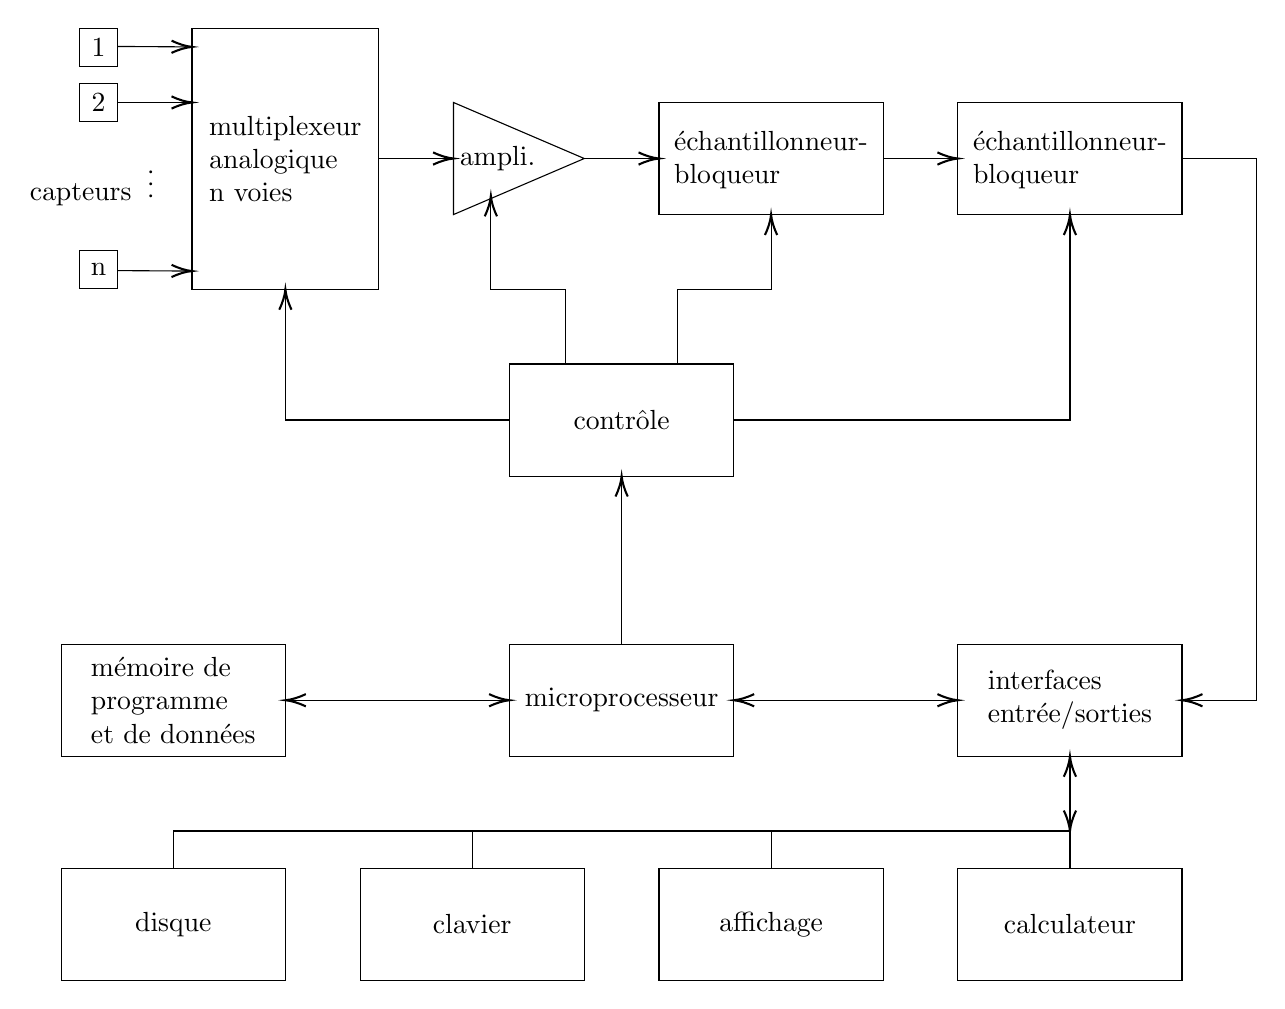
\begin{tikzpicture}[x=0.75pt,y=0.75pt,yscale=-0.9,xscale=0.9]
%uncomment if require: \path (0,542); %set diagram left start at 0, and has height of 542
%https://www.mathcha.io/editor/pJNZQf6yI3nHLEkz1QhWjMp2OT0JYgzyieBJNqK
%Flowchart: Process [id:dp6855416710808666] 
\draw   (110,10.25) -- (210,10.25) -- (210,150) -- (110,150) -- cycle ;
%Shape: Rectangle [id:dp004997227486996603] 
\draw   (50,10.25) -- (70,10.25) -- (70,30.75) -- (50,30.75) -- cycle ;
%Straight Lines [id:da4579113752456023] 
\draw    (70,20) -- (108,20.24) ;
\draw [shift={(110,20.25)}, rotate = 180.36] [color={rgb, 255:red, 0; green, 0; blue, 0 }  ][line width=0.75]    (10.93,-3.29) .. controls (6.95,-1.4) and (3.31,-0.3) .. (0,0) .. controls (3.31,0.3) and (6.95,1.4) .. (10.93,3.29)   ;
%Shape: Rectangle [id:dp6869458093862723] 
\draw   (50,39.75) -- (70,39.75) -- (70,60.25) -- (50,60.25) -- cycle ;
%Straight Lines [id:da4681455266308918] 
\draw    (70,50) -- (108,50) ;
\draw [shift={(110,50)}, rotate = 180] [color={rgb, 255:red, 0; green, 0; blue, 0 }  ][line width=0.75]    (10.93,-3.29) .. controls (6.95,-1.4) and (3.31,-0.3) .. (0,0) .. controls (3.31,0.3) and (6.95,1.4) .. (10.93,3.29)   ;
%Shape: Rectangle [id:dp45817791667488295] 
\draw   (50,129.25) -- (70,129.25) -- (70,149.75) -- (50,149.75) -- cycle ;
%Straight Lines [id:da30660098736037056] 
\draw    (70,140) -- (108,140.24) ;
\draw [shift={(110,140.25)}, rotate = 180.36] [color={rgb, 255:red, 0; green, 0; blue, 0 }  ][line width=0.75]    (10.93,-3.29) .. controls (6.95,-1.4) and (3.31,-0.3) .. (0,0) .. controls (3.31,0.3) and (6.95,1.4) .. (10.93,3.29)   ;
%Straight Lines [id:da6303825397789191] 
\draw    (210,80) -- (248,80) ;
\draw [shift={(250,80)}, rotate = 180] [color={rgb, 255:red, 0; green, 0; blue, 0 }  ][line width=0.75]    (10.93,-3.29) .. controls (6.95,-1.4) and (3.31,-0.3) .. (0,0) .. controls (3.31,0.3) and (6.95,1.4) .. (10.93,3.29)   ;
%Shape: Triangle [id:dp9560439033900896] 
\draw   (320,80) -- (250,110) -- (250,50) -- cycle ;
%Straight Lines [id:da5716448343517799] 
\draw    (320,80) -- (358,80) ;
\draw [shift={(360,80)}, rotate = 180] [color={rgb, 255:red, 0; green, 0; blue, 0 }  ][line width=0.75]    (10.93,-3.29) .. controls (6.95,-1.4) and (3.31,-0.3) .. (0,0) .. controls (3.31,0.3) and (6.95,1.4) .. (10.93,3.29)   ;
%Shape: Rectangle [id:dp5119568810350463] 
\draw   (360,50) -- (480,50) -- (480,110) -- (360,110) -- cycle ;
%Straight Lines [id:da4265953190983147] 
\draw    (480,80) -- (518,80) ;
\draw [shift={(520,80)}, rotate = 180] [color={rgb, 255:red, 0; green, 0; blue, 0 }  ][line width=0.75]    (10.93,-3.29) .. controls (6.95,-1.4) and (3.31,-0.3) .. (0,0) .. controls (3.31,0.3) and (6.95,1.4) .. (10.93,3.29)   ;
%Shape: Rectangle [id:dp7789656892769006] 
\draw   (520,50) -- (640,50) -- (640,110) -- (520,110) -- cycle ;
%Straight Lines [id:da93551183686321] 
\draw    (640,80) -- (680,80) -- (680,370) -- (642,370) ;
\draw [shift={(640,370)}, rotate = 360] [color={rgb, 255:red, 0; green, 0; blue, 0 }  ][line width=0.75]    (10.93,-3.29) .. controls (6.95,-1.4) and (3.31,-0.3) .. (0,0) .. controls (3.31,0.3) and (6.95,1.4) .. (10.93,3.29)   ;
%Shape: Rectangle [id:dp10942318417173202] 
\draw   (280,190) -- (400,190) -- (400,250) -- (280,250) -- cycle ;
%Straight Lines [id:da03354626475894362] 
\draw    (370,190) -- (370,150) -- (420,150) -- (420,112) ;
\draw [shift={(420,110)}, rotate = 450] [color={rgb, 255:red, 0; green, 0; blue, 0 }  ][line width=0.75]    (10.93,-3.29) .. controls (6.95,-1.4) and (3.31,-0.3) .. (0,0) .. controls (3.31,0.3) and (6.95,1.4) .. (10.93,3.29)   ;
%Straight Lines [id:da07083363231785789] 
\draw    (310,190) -- (310,150) -- (270,150) -- (270,102) ;
\draw [shift={(270,100)}, rotate = 450] [color={rgb, 255:red, 0; green, 0; blue, 0 }  ][line width=0.75]    (10.93,-3.29) .. controls (6.95,-1.4) and (3.31,-0.3) .. (0,0) .. controls (3.31,0.3) and (6.95,1.4) .. (10.93,3.29)   ;
%Straight Lines [id:da5566786216518755] 
\draw    (280,220) -- (160,220) -- (160,152) ;
\draw [shift={(160,150)}, rotate = 450] [color={rgb, 255:red, 0; green, 0; blue, 0 }  ][line width=0.75]    (10.93,-3.29) .. controls (6.95,-1.4) and (3.31,-0.3) .. (0,0) .. controls (3.31,0.3) and (6.95,1.4) .. (10.93,3.29)   ;
%Straight Lines [id:da44175483474459487] 
\draw    (400,220) -- (580,220) -- (580,112) ;
\draw [shift={(580,110)}, rotate = 450] [color={rgb, 255:red, 0; green, 0; blue, 0 }  ][line width=0.75]    (10.93,-3.29) .. controls (6.95,-1.4) and (3.31,-0.3) .. (0,0) .. controls (3.31,0.3) and (6.95,1.4) .. (10.93,3.29)   ;
%Straight Lines [id:da4950309462602226] 
\draw    (340,340) -- (340,252) ;
\draw [shift={(340,250)}, rotate = 450] [color={rgb, 255:red, 0; green, 0; blue, 0 }  ][line width=0.75]    (10.93,-3.29) .. controls (6.95,-1.4) and (3.31,-0.3) .. (0,0) .. controls (3.31,0.3) and (6.95,1.4) .. (10.93,3.29)   ;
%Shape: Rectangle [id:dp31894280515360696] 
\draw   (280,340) -- (400,340) -- (400,400) -- (280,400) -- cycle ;
%Shape: Rectangle [id:dp29748923859302145] 
\draw   (520,340) -- (640,340) -- (640,400) -- (520,400) -- cycle ;
%Straight Lines [id:da9319365647593406] 
\draw    (402,370) -- (518,370) ;
\draw [shift={(520,370)}, rotate = 180] [color={rgb, 255:red, 0; green, 0; blue, 0 }  ][line width=0.75]    (10.93,-3.29) .. controls (6.95,-1.4) and (3.31,-0.3) .. (0,0) .. controls (3.31,0.3) and (6.95,1.4) .. (10.93,3.29)   ;
\draw [shift={(400,370)}, rotate = 0] [color={rgb, 255:red, 0; green, 0; blue, 0 }  ][line width=0.75]    (10.93,-3.29) .. controls (6.95,-1.4) and (3.31,-0.3) .. (0,0) .. controls (3.31,0.3) and (6.95,1.4) .. (10.93,3.29)   ;
%Straight Lines [id:da5106166933182902] 
\draw    (162,370) -- (278,370) ;
\draw [shift={(280,370)}, rotate = 180] [color={rgb, 255:red, 0; green, 0; blue, 0 }  ][line width=0.75]    (10.93,-3.29) .. controls (6.95,-1.4) and (3.31,-0.3) .. (0,0) .. controls (3.31,0.3) and (6.95,1.4) .. (10.93,3.29)   ;
\draw [shift={(160,370)}, rotate = 0] [color={rgb, 255:red, 0; green, 0; blue, 0 }  ][line width=0.75]    (10.93,-3.29) .. controls (6.95,-1.4) and (3.31,-0.3) .. (0,0) .. controls (3.31,0.3) and (6.95,1.4) .. (10.93,3.29)   ;
%Shape: Rectangle [id:dp07598328049389613] 
\draw   (40,340) -- (160,340) -- (160,400) -- (40,400) -- cycle ;
%Straight Lines [id:da9982290158431298] 
\draw    (580,460) -- (580,440) -- (100,440) -- (100,460) ;
%Straight Lines [id:da9767066283683422] 
\draw    (260,440) -- (260,460) ;
%Straight Lines [id:da3569597647706805] 
\draw    (420,440) -- (420,460) ;
%Straight Lines [id:da26983482807496484] 
\draw    (580,402) -- (580,438) ;
\draw [shift={(580,440)}, rotate = 270] [color={rgb, 255:red, 0; green, 0; blue, 0 }  ][line width=0.75]    (10.93,-3.29) .. controls (6.95,-1.4) and (3.31,-0.3) .. (0,0) .. controls (3.31,0.3) and (6.95,1.4) .. (10.93,3.29)   ;
\draw [shift={(580,400)}, rotate = 90] [color={rgb, 255:red, 0; green, 0; blue, 0 }  ][line width=0.75]    (10.93,-3.29) .. controls (6.95,-1.4) and (3.31,-0.3) .. (0,0) .. controls (3.31,0.3) and (6.95,1.4) .. (10.93,3.29)   ;
%Shape: Rectangle [id:dp6771105282283583] 
\draw   (40,460) -- (160,460) -- (160,520) -- (40,520) -- cycle ;
%Shape: Rectangle [id:dp09474282891509045] 
\draw   (200,460) -- (320,460) -- (320,520) -- (200,520) -- cycle ;
%Shape: Rectangle [id:dp08838687884544572] 
\draw   (360,460) -- (480,460) -- (480,520) -- (360,520) -- cycle ;
%Shape: Rectangle [id:dp49628749586658394] 
\draw   (520,460) -- (640,460) -- (640,520) -- (520,520) -- cycle ;

% Text Node
\draw (160,80.13) node   [align=left] {multiplexeur\\analogique\\n voies};
% Text Node
\draw (60,20.5) node   [align=left] {1};
% Text Node
\draw (60,50) node   [align=left] {2};
% Text Node
\draw (60,139.5) node   [align=left] {n};
% Text Node
\draw (88,95) node  [rotate=-90] [align=left] {\ldots};
% Text Node
\draw (79,99.5) node [anchor=east] [inner sep=0.75pt]   [align=left] {capteurs};
% Text Node
\draw (252,72) node [anchor=north west][inner sep=0.75pt]   [align=left] {ampli.};
% Text Node
\draw (420,81) node   [align=left] {échantillonneur-\\bloqueur};
% Text Node
\draw (580,81) node   [align=left] {échantillonneur-\\bloqueur};
% Text Node
\draw (340,220) node   [align=left] {contrôle};
% Text Node
\draw (340,370) node   [align=left] {microprocesseur};
% Text Node
\draw (580,370) node   [align=left] {interfaces\\entrée/sorties};
% Text Node
\draw (100,370) node   [align=left] {mémoire de \\programme \\et de données};
% Text Node
\draw (100,490) node   [align=left] {disque};
% Text Node
\draw (260,490) node   [align=left] {clavier};
% Text Node
\draw (420,490) node   [align=left] {affichage};
% Text Node
\draw (580,490) node   [align=left] {calculateur};


\end{tikzpicture}
\end{figure}

Le calculateur associée à la chaine de mesure des fonctions importantes dans la chaine de mesure, elles sont regroupées dans deux catégories :
\begin{itemize}
\item gestion de l'acquisition\,;
\item traitement du signal requis par la précision et la nature de l'information cherchée.
\end{itemize}

Il gère la chaine d'acquisition en délivrant des séquences de signaux de commande. Ceux-ci vont activer de façon ordonnée les dispositifs prévus pour obtenir la valeur du mesurande $m$ :
\begin{enumerate}
\item sélection d'une voie d'entrée par envoie d'adresse au multiplexeur\,;
\item fixation du gain de l'amplificateur programmable\,;
\item échantillonnage puis blocage du signal\,;
\item déclenchement de la conversion analogique-numérique\,;
\item lecture de la donnée numérique à la réception du signal de fin de conversion délivré par le convertisseur analogique-numérique.
\end{enumerate}

En aval de la chaine d'acquisition, le calculateur gère également les périphériques d'entrée-sortie :
\begin{itemize}
\item clavier permettant l'introduction, pour prise en compte par la chaine, d'ordres et de modifications de paramètres de mesure\,;
\item mémoire de masse pour l'archivage des mesures\,;
\item affichage du résultat de la mesure en cours.
\end{itemize}

Les calculateurs permettent aussi d'effectuer des opérations mathématiques sur le signal capté et numérisé :
\begin{itemize}
\item correction du signal reçu\,;
	\begin{itemize}
	\item correction des dérives de zéro et de sensibilité causées par les grandeurs d'influences (en particulier les températures)\,;
	\item correction de la \emph{non-linéarité} des capteurs afin d'obtenir une donnée de sortie proportionnelle au mesurande\,;
	\end{itemize}
\item analyse du signal corrigé.
\end{itemize}



%\end{document}

